\section{Anode Signal Processing}
\label{sec:alct}

\subsection{ALCT Algorithm}
\label{subsec:alct_algo}

Anode wires in CSC are hardwired together at the readout end in groups of 10-15 wires in order to reduce channel count. The anode wire group (WG) signals are fed into the anode front-end boards (AFEBs), each of which contains a single 16-channel amplifier/constant-fraction discriminator chip. The output signals from the AFEBs are sent into the on-chamber ALCT board, which handles triggering and readout of the CSC anode information. Due to the various sizes of CSCs, there are 3 types of ALCT boards, handling 288, 384, and 672 WG channels.

On the ALCT boards, the signals from each AFEB are first delayed by a programmable amount of time in order to perform an average time alignment of the anode signals across the chamber as well as chamber-to-chamber at a sub-bunch crossing level to about 2.2 ns precision. After the AFEB signals are received and time-aligned, then they are latched with bunch crossing frequency and fed to a FPGA (Xilinx Virtex family) mounted on a mezzanine card above the ALCT main board for pattern-finding and readout functions.

The algorithm used in the ALCT FPGA for determining muon segment position and bunch crossing is illustrated below. Since the drift time can be longer than 50 ns, the hits are first stretched by 'one-shots' to 6 BX (150 ns) length. Then, a multi-layer coincidence technique in the ALCT pattern circuitry is used to identify the bunch crossing. For each spatial pattern of anode hits, a low coincidence level, typically 2 or more layers, is used to establish timing, whereas a higher coincidence level, typically 4 layers, is used to establish the existence of a muon track. The general idea of a spatial pattern of CSC wire group hits is illustrated below in Fig.\ref{fig:anode_wire_group_hits}.

\begin{figure}[tbh]
        \begin{center}
                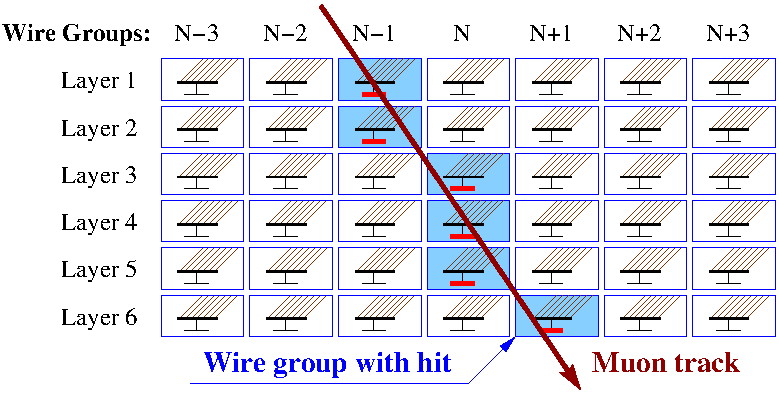
\includegraphics[width=0.6\linewidth]{figures/anode_wire_group_hits.pdf}
                \caption{Illustration of CSC anode wire groups with hits from muon track}
                \label{fig:anode_wire_group_hits}
        \end{center}
\end{figure}

while the general idea of the time stretching of hits, and pretrigger followed by a pattern trigger is shown in Fig.\ref{fig:anode_stretched_hits} (using an example in which one hit is actually missing due to some type of inefficiency).

\begin{figure}[tbh]
        \begin{center}
                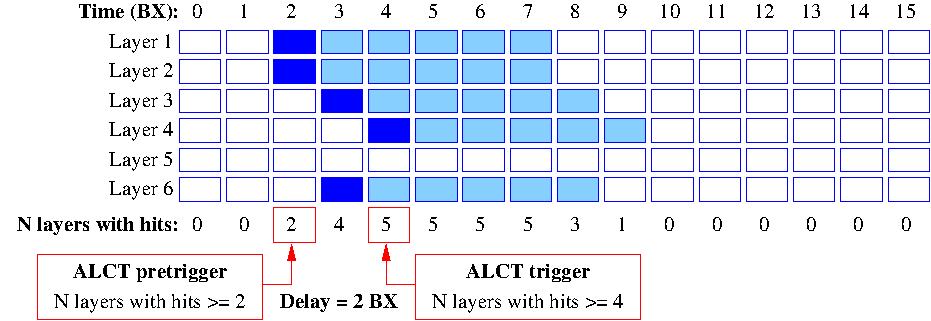
\includegraphics{figures/anode_stretched_hits.pdf}
                \caption{Illustration of anode hits time stretching (6BX) as well as determination of ALCT pretrigger and trigger.}
                \label{fig:anode_stretched_hits}
        \end{center}
\end{figure}

Each pattern detector can detect a programmable "collision" pattern as well as a fixed "accelerator" pattern. The input data for the collision pattern detector are selected as shown below:

\begin{center}
\begin{verbatim}
...n-2 n-1 n...........Layer 1
.......n-1 n...........Layer 2
...........n...........Layer 3
...........n n+1.......Layer 4
...........n n+1 n+2...Layer 5
...........n n+1 n+2...Layer 6
\end{verbatim}
\end{center}

where n in this diagram is the key wire group number, which this particular pattern detector is searching the patterns for. The programming of the programmable collision pattern is implemented as a simple masking-out of the bits that we do not want to include in the pattern. The accelerator pattern is a vertical pattern of 6 layers all with strip n only.

Each ALCT candidate is assigned a quality equal to number of layers with hits minus 3 and passes through a ghost cancellation procedure: it is cancelled if there is another ALCT candidate at the same bunch crossing in the previous wirewith the same or better quality or in the next wire with better quality, or if there is ALCT candidate up to 4 bunch crossing clocks earlier with any quality.

In each bunch crossing two ALCTs with highest quality are sent to the TMB (Trigger MotherBoard), which requires a coincidence between anode and cathode trigger information. In the case of a Level-1 Accept signal from the Global Trigger (distributed via the TTC system to the CCB in each peripheral crate), ALCT data are sequentially transmitted to the Trigger Mother Board and hence to the DAQ Motherboard. These data frames include a few words of ALCT trigger data and a much larger amount of ALCT raw hit data consisting of a time sequence of raw CSC anode wire-group hits that have been stored at the 40 MHz bunch crossing frequence by the ALCT2001. Typically 8 to 16 bunch crossings are read out for each wire group. FIFO data can also be read out much more slowly through VME access via the TMB board using a JTAG electrical interface to the ALCT, if necessary.

For self-monitoring and also for powering and controlling the AFEB cards, the ALCT contains a Slow Control section that supplies power to the AFEBs, controls AFEB thresholds, provides and controls the amplitude of test pulses to the AFEBs, and reads back power supply voltages and currents, as well as on-board temperature. 

\subsection{Improvement of the ALCT Algorithm}
\label{subsec:alct_improvements}

It should be possible to improve the efficiency, rate and timing precision of ALCT stubs by, e.g.
\begin{itemize}
    \item tuning of the ghost cancellation logic (ALCTs in neighboring wiregroups, see "alctGhostCancellationBxDepth" and "alctGhostCancellationSideQuality" parameters in Sec.~\ref{sec:ALCT_conf}) and removing pre-trigger deadtime (see "alctPretrigDeadtime" parameter in Sec.~\ref{sec:ALCT_conf});
    \item using more narrow ALCT pattern in ring 1 chambers (see "alctNarrowMaskForR1" parameter in Sec.~\ref{sec:ALCT_conf});
    \item using more precise algorithm (e.g., running median or truncated average) for BX assignment (see "alctUseCorrectedBx"  parameter in Sec.~\ref{sec:ALCT_conf}).
\end{itemize}

However, here we would only like to focus on how the ALCT stubs would be used by TMB.

ALCTs are reconstructed from the signals in layers of anode wires which are ganged into wiregroups and are continuously covering the whole ME1/1 chamber. Most of the wiregroups can only physically cross only strips either in ME1/1a or only in ME1/1b. A complication specific to ME1/1 is that wires here are not perpendicular to strips, but are slanted at 29 degrees from the straight angle. Thus, some wiregroups are crossing the border between ME1/1a and ME1/1b. If signal is detercted in such a wiregroup, there is an ambiguity about which part of ME1/1 it might belong to.

For the ALCTs received by TMB we propose to split the incoming stubs into two parts, ME1/1a and ME1/1b, that would be used further for LCT matching separately in ME1/1a and ME1/1b. 




\subsection{Emulation of ALCT Algorithm}
\label{subsec:alct_emulation}

ALCT processing includes the following five steps:

\begin{itemize}
    \item Pulse extension;
    \item Pretrigger;
    \item Trigger;
    \item Ghost cancellation;
    \item ALCT construction.
\end{itemize}

\subsubsection{Pulse Extension}

Sofware emulation provides information about all wire signals in DAQ readout window (16 BXs). A search for these signals is performed in a loop over all wire groups, all layers, and all 16 BXs; found signals are stretched over 6 BXs (see Fig.~\ref{fig:alct_pulse_extension}).

\begin{figure}[tbh]
        \begin{center}
                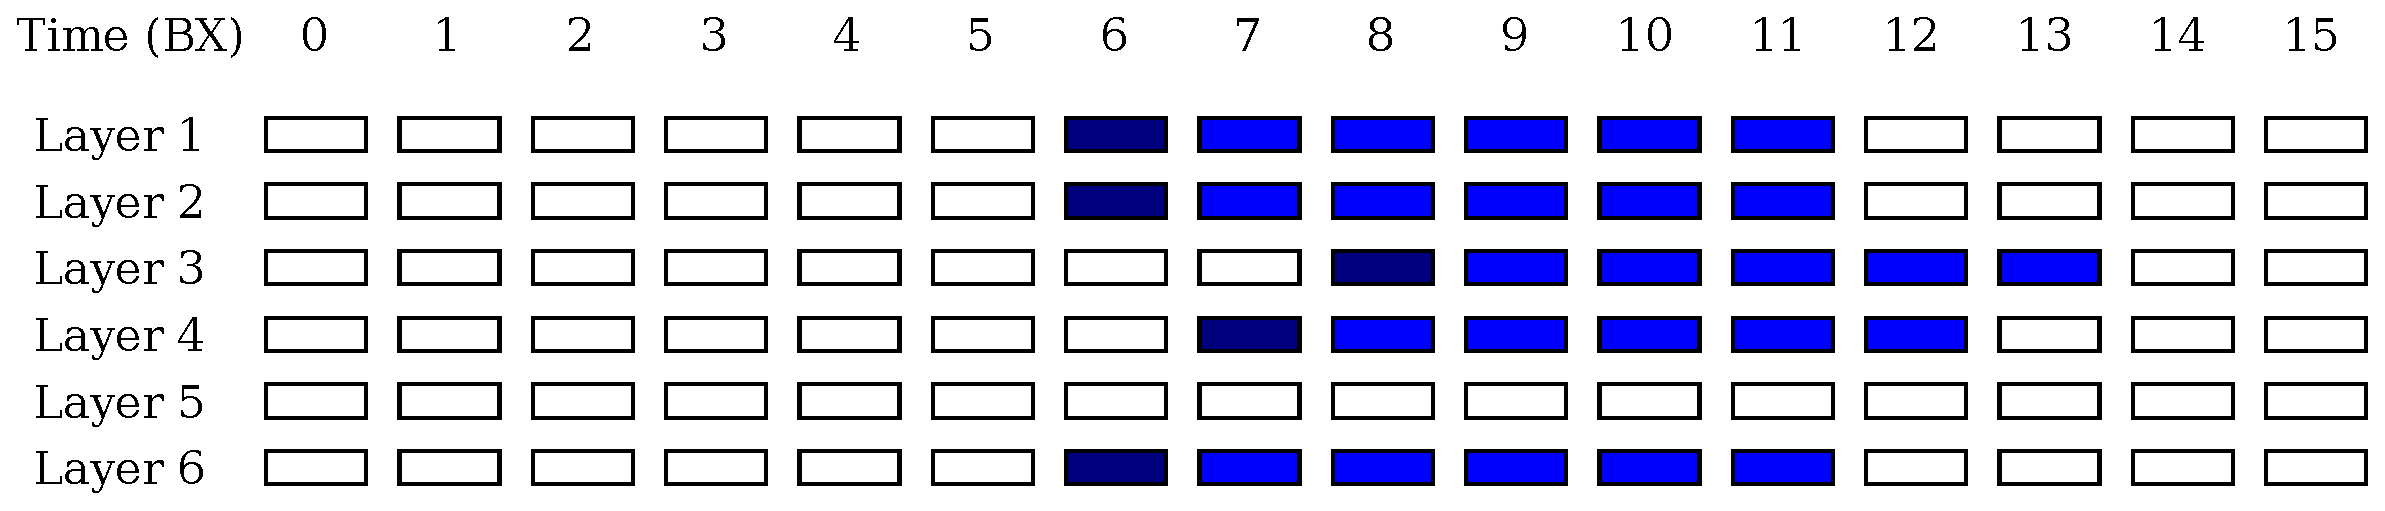
\includegraphics[width=0.9\linewidth]{figures/stretched_hits_alct.pdf}
                \caption{Illustration of ALCT pulse extension for one specific wire group.}
                \label{fig:alct_pulse_extension}
        \end{center}
\end{figure}

\subsubsection{Pretrigger}

After all available wire signals are stretched, a search for ALCT pretriggers is performed in all wire groups and all BXs. For any given wire group and BX, we count the number of layers with hits within the pattern mask shown on Fig.~\ref{fig:alct_pretrigger}, and if this number is greater than or equal to three, then we say that a pretrigger occured in this wire group and BX. The search for next ALCT pretrigger starts 6 BXs later.

\begin{figure}[tbh]
        \begin{center}
                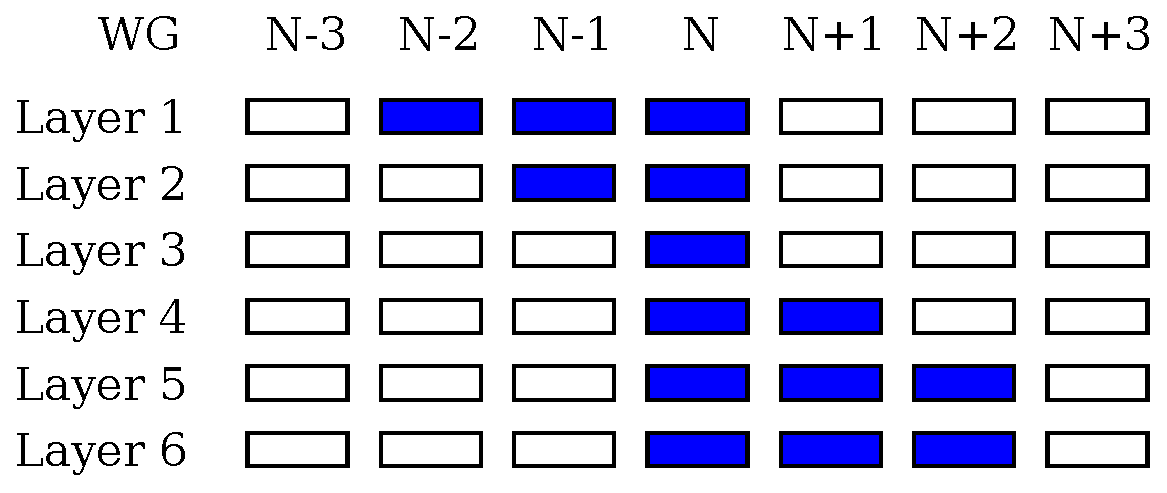
\includegraphics[width=0.45\linewidth]{figures/alct_pretrigger.pdf}
                \caption{ALCT pattern mask for pretriggering and triggering.}
                \label{fig:alct_pretrigger}
        \end{center}
\end{figure}

\subsubsection{Trigger}

After all ALCT pretriggers are found, for each pretrigger in BX = B we check for a trigger in BX = B+2. For any given wire group and BX = B+2, we count the number of layers with hits within the same pattern mask used for pretriggering, and if this number is greater than or equal to four, we say that a pretrigger occured in this wire group and BX, and assign it a quality Q = number of layers with hits-3. If in some wire group more than one trigger occured, we report only the one with the highest quality. If there are two triggers with the same quality, report the earlier one.

\subsubsection{Ghost Cancellation}

Not all triggers found in the previous step are used to construct ALCTs: before that all of them pass through so called ghost cancellation procedure.

A trigger in wire group = N and BX = B is cancelled if there is a trigger in wire group = N-1:
\begin{itemize}
    \item either in the same BX = B and with better or equal quality;
    \item or to 4 BXs earlier, with any quality.
\end{itemize}

In addition, a trigger in wire group = N and BX = B is cancelled if there is a trigger in wire group = N+1:
\begin{itemize}
    \item either in the same BX = B and with better quality;
    \item or to 4 BXs earlier, with any quality.
\end{itemize}

\subsubsection{ALCT Construction}

Construct ALCTs from triggers survived after the ghost cancellation procedure: encode quality, WG, BX (defined by pretrigger BX). In every BX choose best two ALCTs: two ALCTs with the highest quality. If we need to choose one ALCT from two ALCTs with the same quality: choose the one with larger wire group.


\subsection{Sofware Emulation of ALCT Level Improvements}

\subsubsection{Tuning of Ghost Cancellation Procedure}

\textcolor{red}{Current} ghost cancellation:
\begin{itemize}
    \item Loop over wire groups:
    \begin{itemize}
        \item Consider WG = N
        \item Cancel trigger in this wire group if there is trigger in WG = N-1 and:
        \begin{itemize}
            \item with the same BX and with \textcolor{red}{better or equal} quality
            \item up to \textcolor{red}{4} BXs earlier, with \textcolor{red}{any} quality
        \end{itemize}
        \item Cancel trigger in this wire group if there is trigger in WG = N+1 and:
        \begin{itemize}
            \item with the same BX and with \textcolor{red}{better} quality
            \item up to \textcolor{red}{4} BXs earlier, with \textcolor{red}{any} quality
        \end{itemize}
    \end{itemize}
\end{itemize}
\textcolor{blue}{New} ghost cancellation:
\begin{itemize}
    \item Loop over wire groups:
    \begin{itemize}
        \item Consider WG = N
        \item Cancel trigger in this wire group if there is trigger in WG = N-1 and:
        \begin{itemize}
            \item with the same BX and with \textcolor{blue}{better} quality
            \item up to \textcolor{blue}{1} BX earlier, with \textcolor{blue}{better} quality
        \end{itemize}
        \item Cancel trigger in this wire group if there is trigger in WG = N+1 and:
        \begin{itemize}
            \item with the same BX and with \textcolor{blue}{better or equal} quality
            \item up to \textcolor{blue}{1} BX earlier, with \textcolor{blue}{better and equal} quality
        \end{itemize}
    \end{itemize}
\end{itemize}

The following modifications in configuration are related to this improvement:
\begin{itemize}
    \item alctGhostCancellationBxDepth: 4BX to 1BX
    \item alctGhostCancellationSideQuality: False to True
\end{itemize}

\subsubsection{Narrow ALCT Pattern Mask}

Use more narrow ALCT pattern mask for stations in Ring 1 (see Fig.~\ref{fig:narrow_alct_pattern_mask}).

\begin{figure}[tbh]
        \begin{center}
                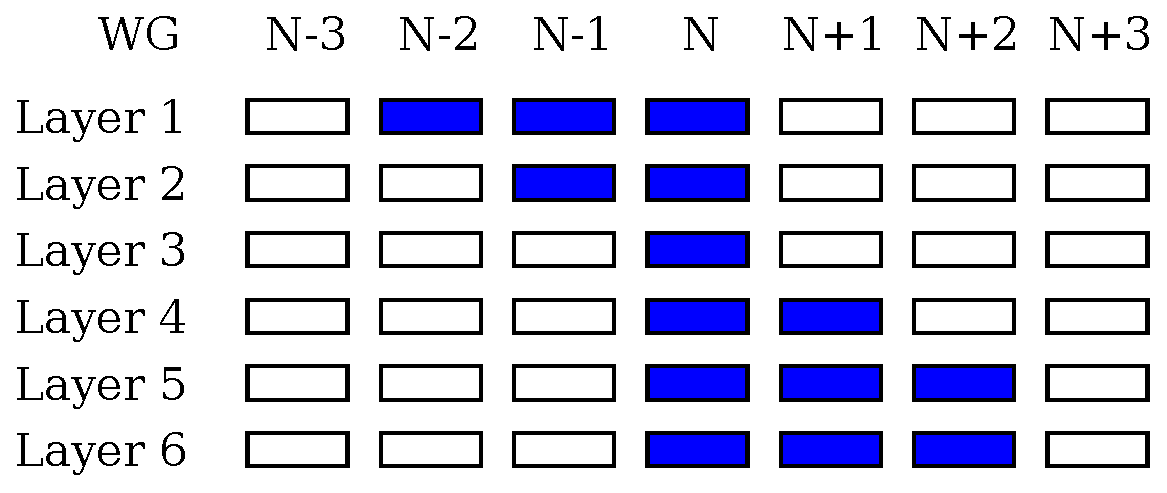
\includegraphics[width=0.49\linewidth]{figures/alct_pretrigger.pdf}\\
                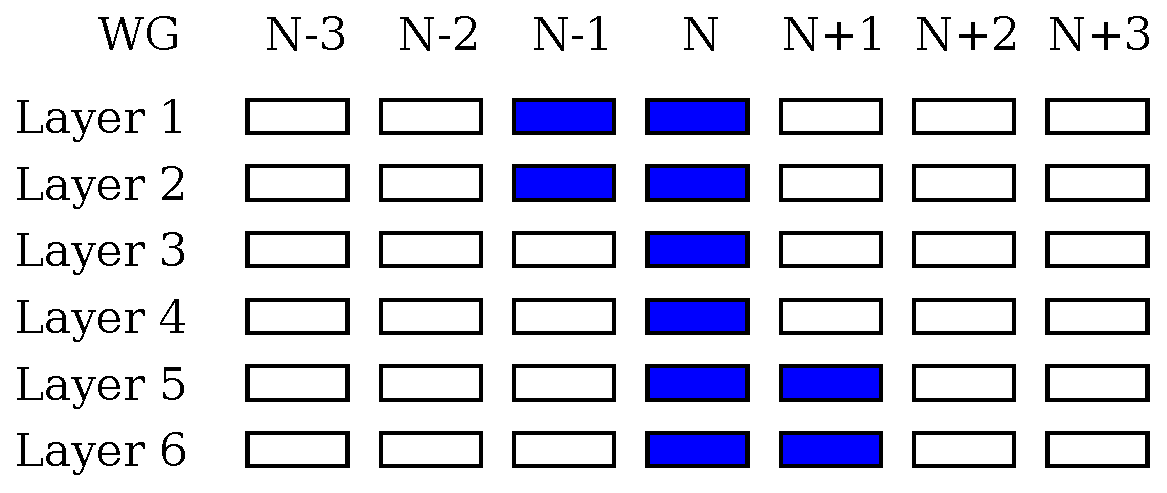
\includegraphics[width=0.49\linewidth]{figures/alct_pretrigger_r1.pdf}
                \caption{Top: default ALCT pattern mask, bottom: narrow ALCT pattern mask.}
                \label{fig:narrow_alct_pattern_mask}
        \end{center}
\end{figure}

The following modifications in configuration are related to this improvement:
\begin{itemize}
    \item alctNarrowMaskForR1: False to True
\end{itemize}

\subsubsection{Reduced ALCT Dead Time}

Currently, if there is pretrigger in BX = B (see Fig.~\ref{fig:alct_deadtime}):
\begin{itemize}
    \item Check for trigger in BX = B + drift time = B+2
    \item Search for next pretrigger starting from BX = B + drift time + extra deadtime = B+6
\end{itemize}

Suggested improvement: decrease extra deadtime from 4 BX to 0 BX.

\begin{figure}[tbh]
        \begin{center}
                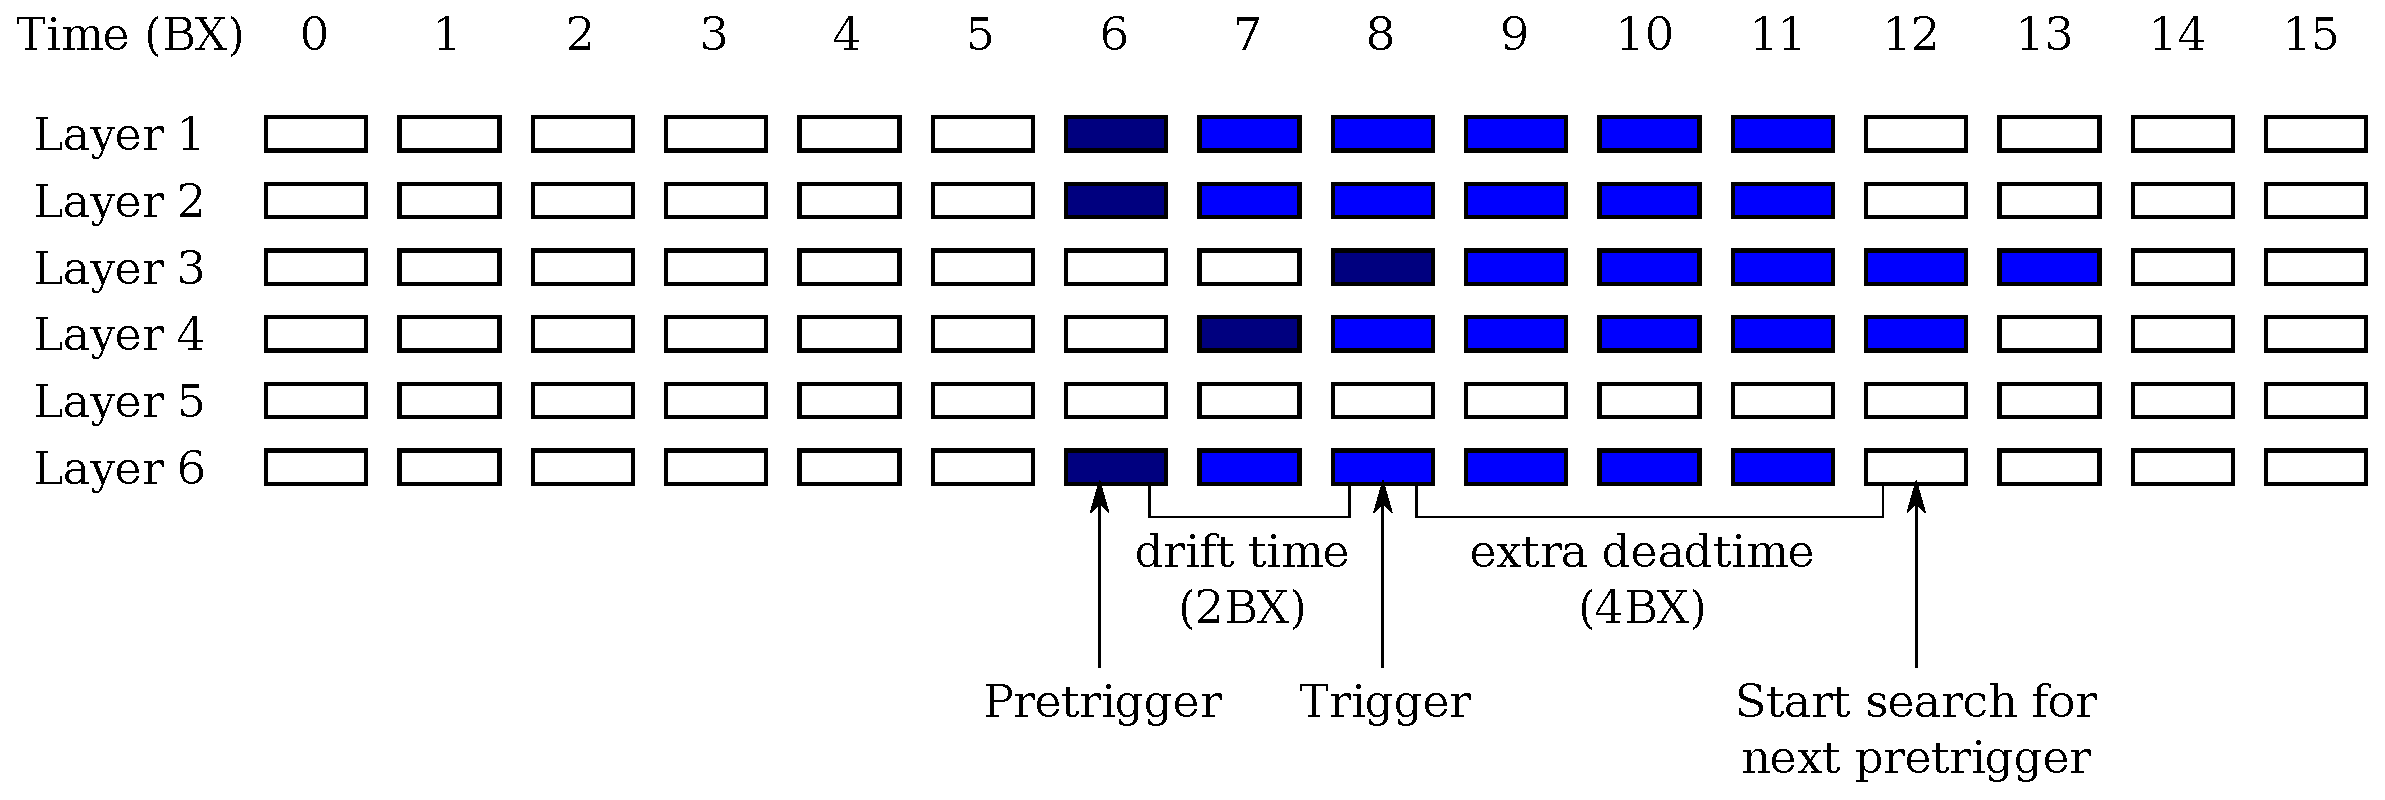
\includegraphics[width=0.98\linewidth]{figures/stretched_hits_alct_deadtime.pdf}
                \caption{Top: Dead Time between ALCT pretriggers.}
                \label{fig:alct_deadtime}
        \end{center}
\end{figure}

The following modifications in configuration are related to this improvement:
\begin{itemize}
    \item alctPretrigDeadtime: 4BX to 0BX
\end{itemize}


\subsection{Results of Improvements of the ALCT Processing}

Improvements on the level of ALCT processor are related to the following configuration parameters (see Sec.~\ref{sec:ALCT_conf}):
\begin{itemize}
	\item alctGhostCancellationBxDepth: 4BX to 1BX;
	\item alctGhostCancellationSideQuality: False to True;
	\item alctNarrowMaskForR1: False to True;
	\item alctPretrigDeadtime: 4BX to 0BX.
\end{itemize}

Fig.~\ref{fig:ALCT_improvements_ALCT_recoEff} shows reconstruction efficiency of a good ALCT in ME1/1 station versus pseudorapidity of the simulated muon for different L1 configurations. The good ALCT is defined as ALCT:
\begin{itemize}
	\item read out in the window of 3BX around the central BX (BX6);
	\item reconstructed within 2 anode wire groups from the key wire group.
	\item has hits at least on four layers
\end{itemize}

The major improvement in ALCT reconstruction efficiency comes from the changes in ALCT ghost cancellation procedure.

\begin{figure}[p]
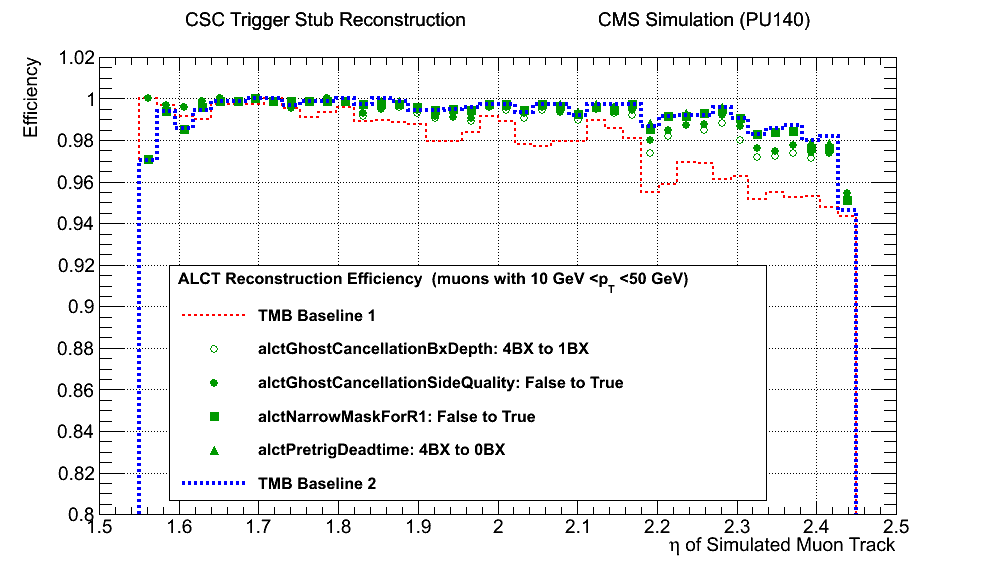
\includegraphics[width=0.98\textwidth]{figures/ALCT_improvements_ALCT_recoEff.png}
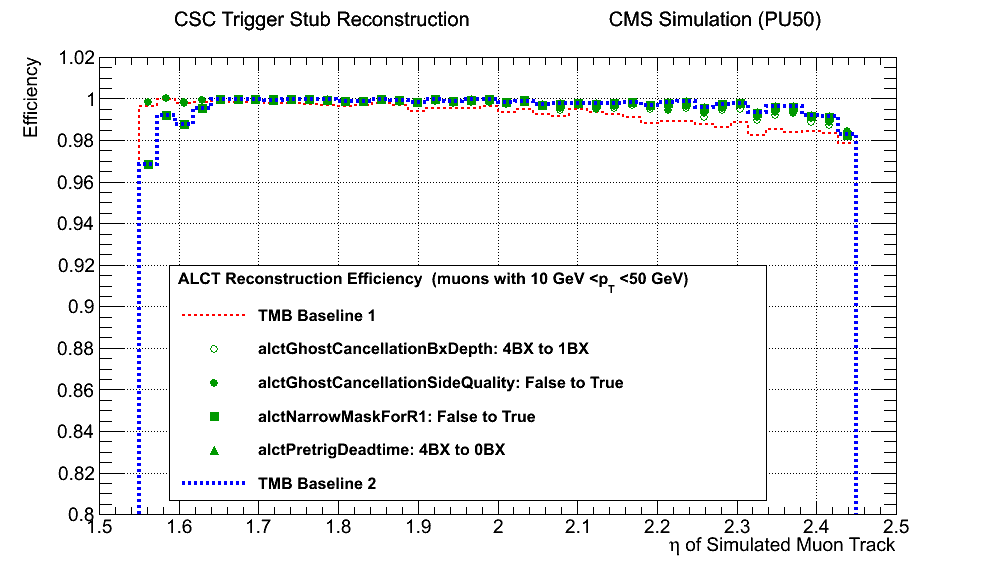
\includegraphics[width=0.98\textwidth]{figures/ALCT_improvements_ALCT_recoEff_PU50.png}
\caption{ALCT reconstruction efficiency in ME1/1 station for PU140 (top) and PU50 (bottom). Muons with transverse momentum $10$~GeV$<p_T<50$~ GeV are used in the analysis.}
\label{fig:ALCT_improvements_ALCT_recoEff}
\end{figure}